
\section{\ours: A Simple and Plain Detector}
\label{sec:simplr}

Multi-scale feature maps in a hierarchical backbone can be easily extracted from the pyramid structure~\cite{wei2016ssd,tsung2017fpn,zhu2021deformable}. When moving to a ViT backbone with a constant feature resolution, the creation of multi-scale feature maps requires complex backbone adaptations. Moreover, the benefits of multi-scale features in object detection frameworks using ViTs remain unclear. Recent studies on plain-backbone detection~\cite{li2022vitdet,chen2022uvit} conjecture the high-dimensional ViT with self-attention and positional embeddings~\cite{vaswani2017transformer} is able to preserve important information for localizing objects\footnote{ViT-B and larger ($\text{dim}\ge768$) can maintain information with a patch size of $16{\times}16{\times}3$ in the input image.}. From this conjecture, we hypothesize that a proper design of the transformer-based head will enable a plain detector.

Our proposed detector, \ours, is conceptually simple: a pre-trained ViT backbone to extract plain features from an image, which are then fed into a single-scale encoder-decoder to make the final prediction (See \cref{fig:compare}). Thus, \ours is a natural idea as it eliminates the non-trivial creation of feature pyramids from the ViT backbone. But the single-scale encoder-decoder requires an effective design to deal with objects at different scales. First, we review box-attention in \cite{nguyen2022boxer} as our baseline in end-to-end detection and segmentation using feature pyramids. Then, we introduce the key elements of our plain detector, \ours, including its \emph{scale-aware} attention that is the main factor for learning of adaptive object scales.

\subsection{Background}

Our goal is to further simplify the detection and segmentation pipeline from~\cite{zhu2021deformable,li2022vitdet,nguyen2022boxer}, and to prove the effectiveness of the plain detector in \textit{both} object detection and segmentation tasks. As a result, we utilize the sparse attention mechanism, box-attention in~\cite{nguyen2022boxer}, as strong baselines due to its effectiveness in learning discriminative object representations while being lightweight in computation.

In box-attention, each query vector $q \in \mathbb{R}^d$ in the input feature map is assigned a reference window $r {=} [x, y, w, h]$, where $x, y$ indicate the query coordinate and $w, h$ are the size of the reference window. The box-attention refines the reference window into a region of interest.
During the attention head computation, a $2 {\times} 2$ feature grid is sampled from the corresponding region of interest, resulting in a set of value features $v_i \in \mathbb{R}^{2 \times 2 \times d_h}$. The $2 {\times} 2$ attention scores are efficiently generated by computing a dot-product between $q \in \mathbb{R}^d$ and relative position embeddings ($k_i \in \mathbb{R}^{2 \times 2 \times d}$) followed by a $\softmax$ function. The attended feature $\mathrm{head}_i \in \mathbb{R}^{d_h}$ is a weighted sum of $2 {\times} 2$ value features in $v_i$ with the corresponding attention weights:
%
% \begin{equation}
%     \alpha =  \softmax(q^{\top} {k_i}),
% \end{equation}
% \begin{equation}
%     \mathrm{head}_i = \mathop{\mathrm{\boxattnop}}(q, k_i, v_i) = \sum_{j=0}^{2 \times 2} \alpha_j v_{i_j},
% \end{equation}
%
To capture objects at different scales, the box-attention~\cite{nguyen2022boxer} takes $t$ multi-scale feature maps, $\{e^j\}_{j=1}^t$, as its inputs in order to produce $\mathrm{head}_i$. The multi-scale box-attention shows strong performance in end-to-end object detection and instance segmentation.

The sparse attention like box-attention lies at the core of recent end-to-end detection and segmentation models due to its ability of capturing object information with lower complexity. The effectiveness and efficiency of these attention mechanisms bring up the question: \textit{Is multi-scale object information learnable within the detector which is non-hierarchical and single-scale?}

\subsection{Scale-aware attention}

The output features of the encoder should capture objects at different scales. Therefore, unlike the feature pyramids where each set of features encode a specific scale, predicting objects from a plain feature map requires its feature vectors to reason about dynamic scale information based on the image content. This can be addressed effectively by a multi-head attention mechanism that capture different scale information in each of its attention heads. 
In that case, global self-attention is a potential candidate because of its large receptive field and powerful representation. However, its computational complexity is quadratic \wrt the sequence length of the input, making the operation computationally expensive when dealing with high-resolution images. The self-attention also leads to worse performance and slow convergence in end-to-end detection~\cite{zhu2021deformable}. This motivated us to develop a multi-head \emph{scale-aware} attention mechanism for single-scale input.

\boldparagraph{Scale-aware attention.} In the sparse attention mechanism such as deformable attention~\cite{zhu2021deformable} or box-attention~\cite{nguyen2022boxer}, each feature vector is assigned to a single scale in feature pyramids. As a result, feature vectors learn to adapt to that specific scale assigned to them. While this behaviour may not impact the multi-scale deformable attention or box-attention -- which utilizes feature pyramids for detecting objects -- it poses a big challenge in learning scale-equivariant features on a single-scale input.

To address this limitation, we propose two variants of multi-head \emph{scale-aware} attention (\ie, \emph{fixed-scale} and \emph{adaptive-scale}) that integrate different scales into each attention head, allowing query vectors to choose the suitable scale information during training. Our proposed attention mechanism is simple: we assign reference windows of $m$ different scales to attention heads of each query. We use $m$ reference windows with size $w {=} h \in \{s \cdot 2^j\}_{j=0}^{m-1}$, where $s$ is the size of the smallest window, and $m$ is the number of scales. Surprisingly, our experiments show that the results are \emph{not} sensitive to the size of the window, as long as \emph{enough number of scales} are used.
%
\begin{enumerate}[leftmargin=*,itemsep=0pt,topsep=0pt]
    \item[i)] \emph{Fixed-Scale Attention.} Given reference windows of $m$ scales, we distribute them to $n$ attention heads in a round-robin manner. Thus, in multi-head fixed-scale attention, $\frac{n}{m}$ attention heads are allocated for each of the window scales. This uniform distribution of different scales enables fixed-scale attention to learn diverse information from local to more global context. The aggregation of $n$ heads results in scale-aware features, that is suitable for predicting objects of different sizes.
    \item[ii)] \emph{Adaptive-Scale Attention.} Instead of uniformly assigning $m$ scales to $n$ attention heads, the adaptive-scale attention learns to allocate a scale distribution based on the context of the query vector. This comes from the motivation that the query vector belonging to a small object should use more attention heads for capturing fine-grained details rather than global context, and vice versa. 
    
    % More specifically, in each attention head, the adaptive-scale attention predicts offsets for all reference windows of $m$ scales and samples feature grids from $m$ regions-of-interest. 
    % Given the query vector $q \in \mathbb{R}^d$, it then applies a learnable projection on $q$ followed by $\softmax$ normalization to generate attention scores which allow it to focus on the feature grid of suitable scale. The adaptive-scale attention provides efficiency due to sparse sampling and strong flexibility to control scale distribution via its attention computation.
    Given the query vector $q \in \mathbb{R}^d$ in the input feature map and $m$ reference windows of different scales, $\{r^j\}_{j=0}^{m-1}$, the adaptive-scale attention predicts offsets of all reference windows, $\{\Delta_{x_j},\Delta_{y_j},\Delta_{w_j},\Delta_{h_j}\}_{j=0}^{m-1}$, in each attention head. Besides, we apply a scale temperature to each set of offsets before the transformations:
    \begin{equation}
        F_\text{scale}(r_j, q) = [x, y, w + \Delta_w\cdot\frac{2^j}{\lambda}, h + \Delta_h\cdot\frac{2^j}{\lambda}], 
    \end{equation}
    \begin{equation}
        F_\text{translate}(r_j, q) = [x + \Delta_x\cdot\frac{2^j}{\lambda}, y + \Delta_y\cdot\frac{2^j}{\lambda}, w, h],
    \end{equation}
    where $\frac{2^j}{\lambda}$ is the scale temperature corresponding to $r_j$. The scale temperature allows the transformation functions to capture regions of interest corresponding to the scale of reference windows. It then samples feature grids from $m$ regions of interest and generates attention scores for these feature grids followed by $\softmax$ normalization. This makes our attention mechanism to focus on feature grids of suitable scale. The adaptive-scale attention provides efficiency due to sparse sampling and strong flexibility to control scale distribution via its attention computation.
\end{enumerate}

\subsection{Object Representation for Panoptic Segmentation} 

Panoptic segmentation proposed by~\cite{kirillov2019panoptic} requires the network to segment both ``thing'' and ``stuff''. To enable the plain detector on panoptic segmentation, we make an adaptation in the mask prediction of \ours. Following~\cite{cheng2022mask2former}, we predict segmentation masks of both types by computing the dot-product between object queries and a high-resolution feature map (\ie, $\frac{1}{4}$ feature scale).

As the ViT and SimPLR encoder features are of lower resolution, we simply interpolate the last encoder layer to $\frac{1}{4}$ scale and add a single scale-aware attention layer on top. This simple modification produces a high resolution feature map that is beneficial for learning fine-grained details.

\begin{figure}[t]
\floatbox[{\capbeside\thisfloatsetup{capbesideposition={right,top},capbesidewidth=4cm}}]{figure}[\FBwidth]
{\caption{
    \textbf{Masked Instance-Attention. Left:} The box-attention~\cite{nguyen2022boxer} which samples $2\times2$ grid features in the region of interest. \textbf{Right:} Our masked instance-attention for dense grid sampling. The $2\times2$ attention scores are denoted in four colours and the masked attention scores are in white.}
    \label{fig:masked_instance_attn}}%
{
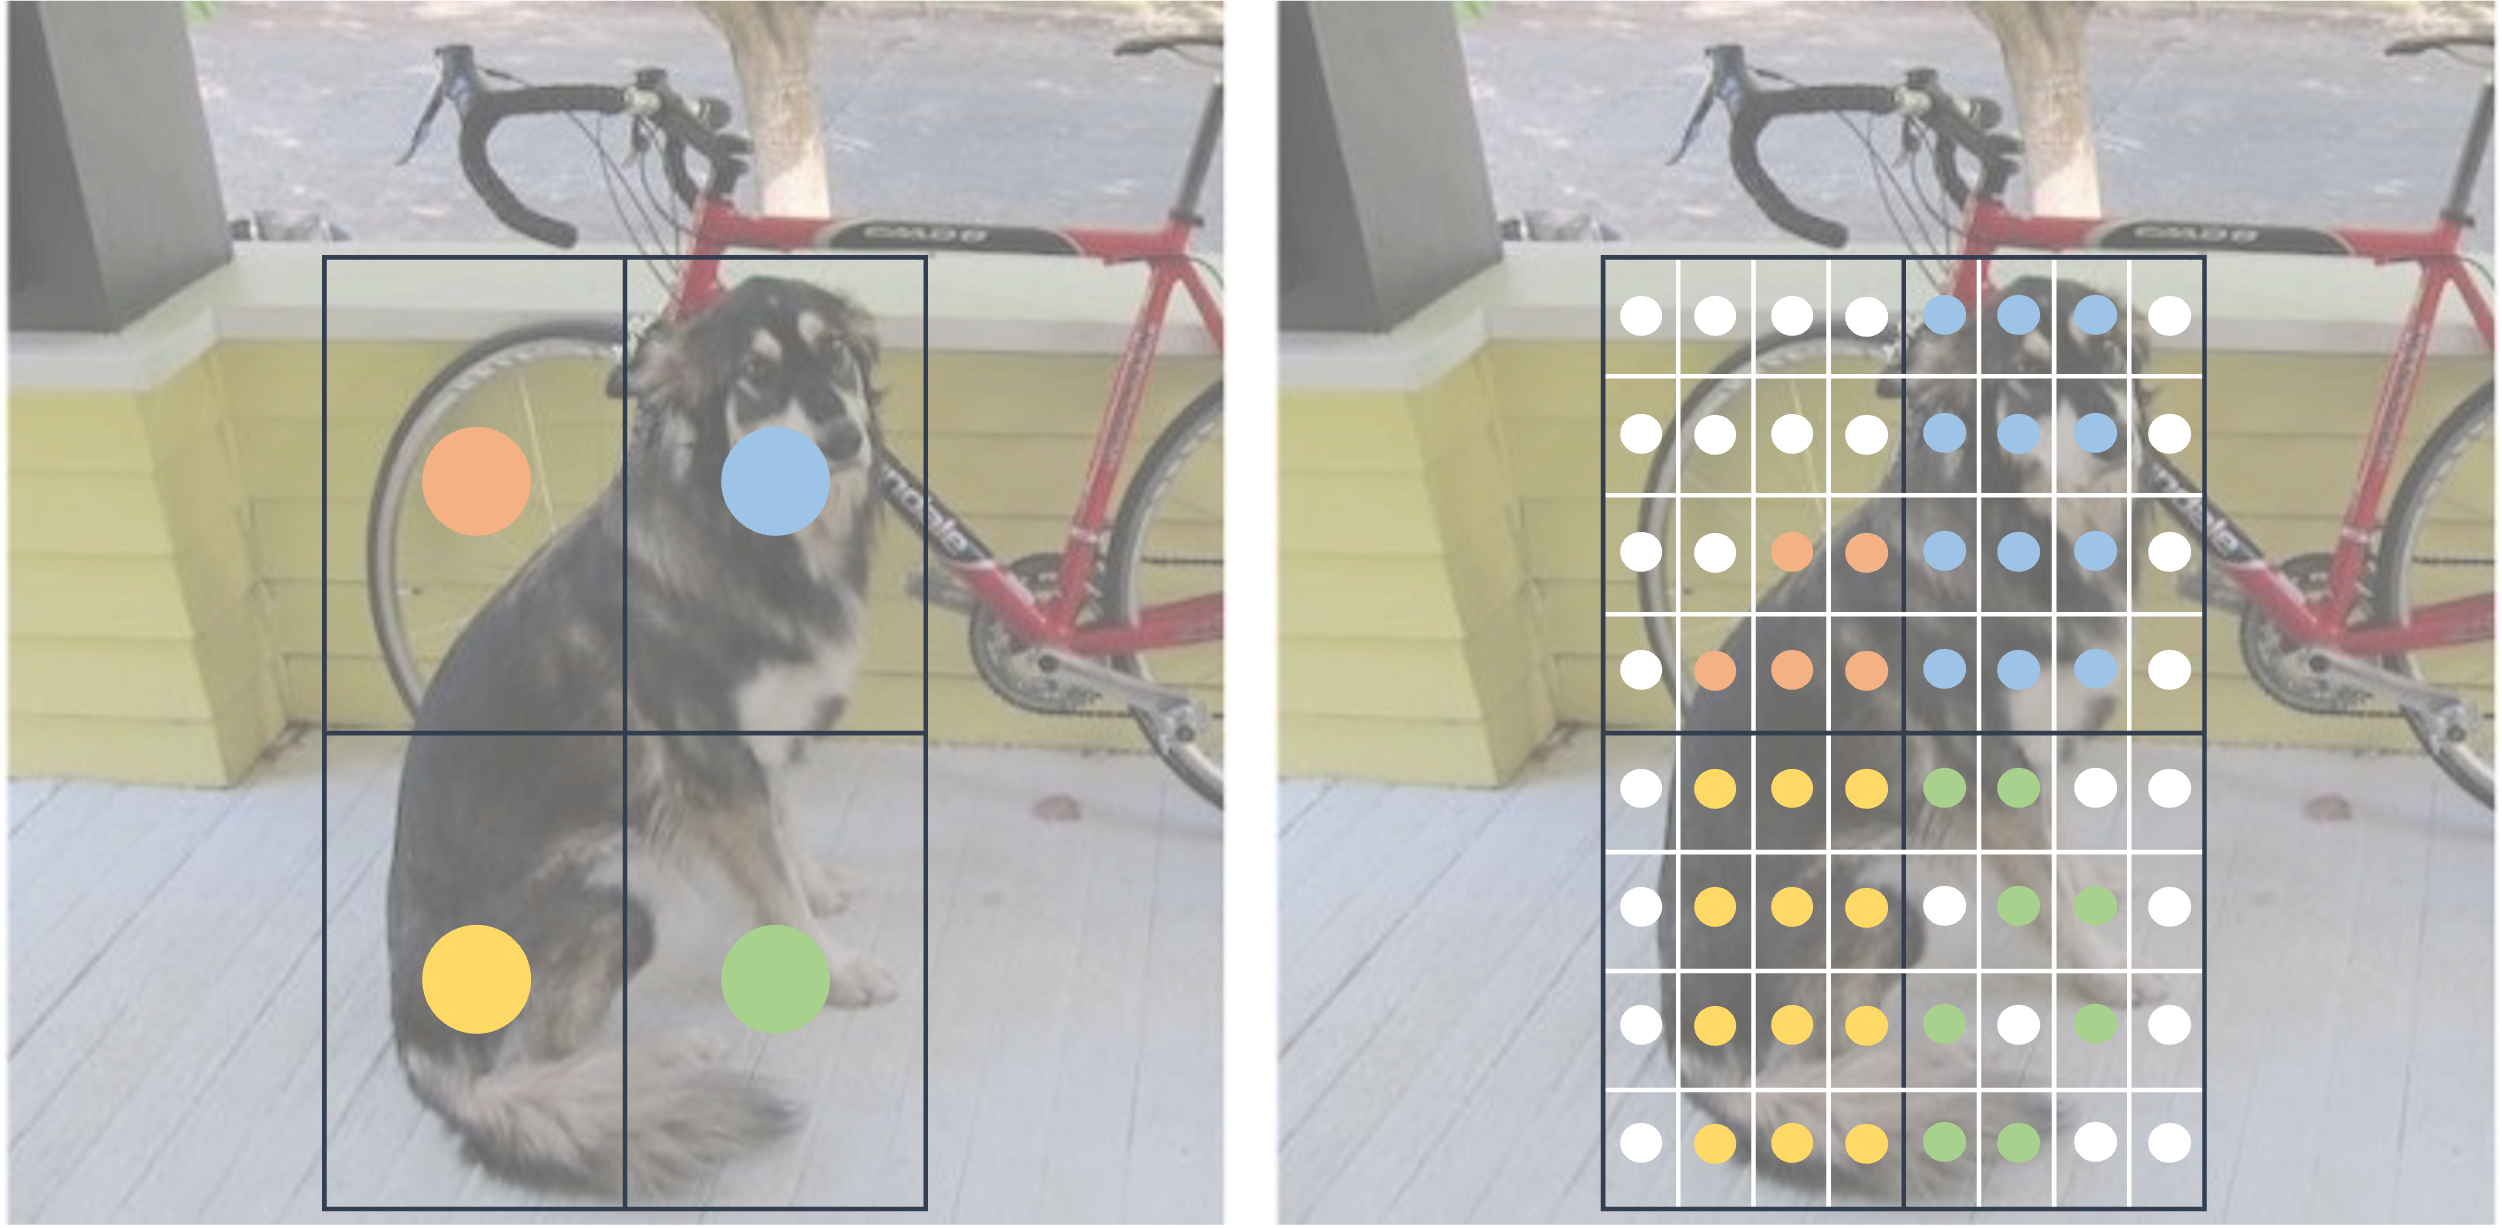
\includegraphics[width=7.5cm]{fig/attn_comp.png}
}
\end{figure}

\boldparagraph{Masked instance-attention.} In order to learn better object representation in the decoder, we propose masked instance-attention that is also a sparse attention mechanism for efficiency. The masked instance-attention follows the grid sampling strategy of the box-attention in~\cite{nguyen2022boxer}, but improves the attention computation to better capture objects of
different shapes.

To be specific, the region of interest $r'_i$ is divided into 4 bins of $2 \times 2$ grid, each of which contains a $\frac{m}{2} \times \frac{m}{2}$ grid features sampled using bilinear interpolation. Instead of assigning an attention weight to each feature vector, a linear projection ($\mathbb{R}^d \rightarrow \mathbb{R}^{2 \times 2}$) is adopted to generate the $2 \times 2$ attention scores for 4 bins. The $\frac{m}{2} \times \frac{m}{2}$ feature vectors within the same bin share the same attention weight. Inspired by \cite{cheng2022mask2former}, we utilize the mask prediction of the previous decoder layer as the attention mask to guide the attention scores to better capture the boundary of objects (see \cref{fig:masked_instance_attn}).
\begin{equation}
    \mathrm{head}_i = \sum_{k=0}^{2 \times 2} \sum_{j=0}^{\frac{m}{2} \times \frac{m}{2}} \frac{\alpha_k}{\frac{m}{2} \cdot \frac{m}{2}} \, v_{i_{k,j}},
\end{equation}
where $a_k$ is the attention weight corresponding to $k$-th bin, $v_{i_{k,j}}$ is the $j$-th feature vector inside $k$-th bin.

\subsection{Network Architecture}

\ours follows the end-to-end detection and segmentation framework in~\cite{nguyen2022boxer} with the two-stage design. Specifically, we use a plain ViT as the backbone with $14\times14$ windowed attention and four equally-distributed global attention blocks as in~\cite{li2022vitdet}. In the detection head, the \ours encoder receives input features via a projection of the last feature map from the ViT backbone. The object proposals are then generated using single-scale features from the encoder and top-scored features are initialized as object queries for the \ours decoder to predict bounding boxes and masks. 

Formally, we apply a projection $f$ to the last feature map of the pre-trained ViT backbone, resulting in the input feature map $e \in \mathbb{R}^{H_e \times W_e \times d}$ where $H_e, W_e$ are the size of the feature map, and $d$ is the hidden dimension of the detection head. In \ours, the projection $f$ is simply a single convolution projection, that provides us a great flexibility to control the resolution and dimension of the input features $e$ to the encoder. The projection allows \ours to decouple the feature scale and dimension between its backbone and detection head to further improve the efficiency. This practice is different from the creation of SimpleFPN in~\cite{li2022vitdet} where a different stack of multiple convolution layers is used for each feature scale (more details shown in Fig. A in the supplementary material). We show by experiments that this formulation is key for plain detection and segmentation while keeping our network efficient.

\boldparagraph{Plain backbone.} \ours deploys ViT as its plain backbone for feature extraction. We show that \ours can take advantages of recent progress in self-supervised learning with ViTs. To be specific, \ours generalizes to ViT backbones initialized by MAE~\cite{he2022mae} and BEiTv2~\cite{peng2022beitv2}. The efficient design of \ours allows us to effectively scale to larger ViT backbones which recently show to be even more powerful in learning representations~\cite{he2022mae,zhai2022scalingvit,dehghani2023scalingvit22b}. We provide more details in the supplementary material.
